\section{Конструкторская часть}

В данном разделе переставлена архитектура программного обеспечения (модуля ядра zram). Приведен алгоритм вычисления информационной энтропии для страниц оперативной памяти и алгоритм записи страниц в блочном устройстве.

Алгоритмы рассчитаны на организацию кода в блоки, в которых могут быть несколько точек выхода и одна точка входа.

\subsection{Архитектура программного обеспечения}

На рисунке \ref{fig:zram-archeticture} представлена архитектура блочного устройства zram (в виде вызываемых функций).

\begin{figure}[h]
	\centering
	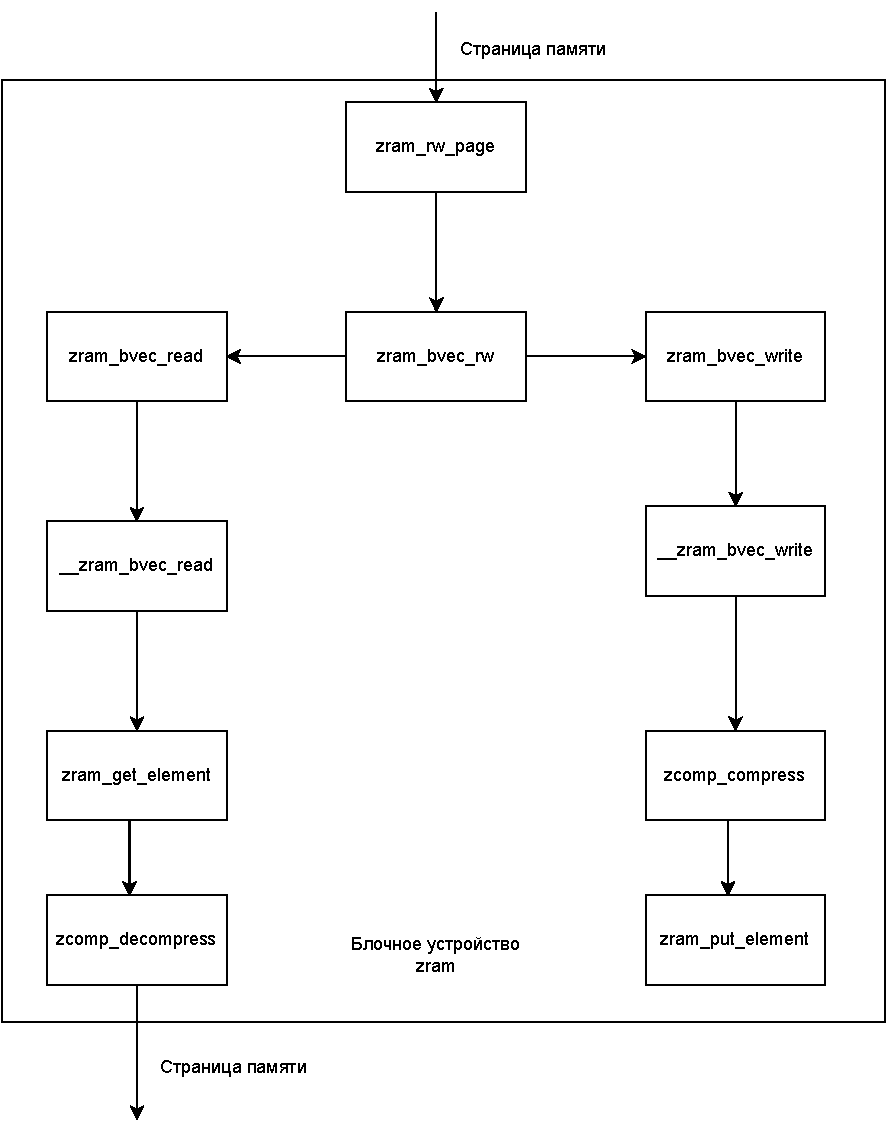
\includegraphics[scale=1]{img/zram-arch.pdf}
	\caption{Архитектура модуля ядра zram}
	\label{fig:zram-archeticture}
\end{figure}

Ниже приведено описание каждой из функций, представленных на рисунке \ref{fig:zram-archeticture}:

\begin{itemize}
	\item zram\_rw\_page() -- эта функция является точкой входа для каждой страницы попавшей в блочное устройство. В этой функции происходят подготовительные вызовы: например, уведомление о начале I/O операции. После выполнения всех подготовительных операций, вызывается функция zram\_bvec\_rw();
	\item zram\_bvec\_rw() -- в зависимости от операции, которую необходимо произвести прочитать сжатую страницу из блочного устройства или сжать и сохранить страницу, в этой функции вызывается функция zram\_bvec\_rw() или zram\_bvec\_write() соответственно;
	\item zram\_bvec\_read() -- эта функция является обёрткой над функцией \\\_\_zram\_bvec\_read(). Выполняет некоторые подготовительные действия и вызывает следующую функцию.
	\item \_\_zram\_bvec\_read() --поиск индекса необходимой страницы, которую нужно вернуть, в блочном устройстве, вызов функции \\zram\_get\_element();
	\item zram\_get\_element() -- возвращает сжатую страницу, хранящуюся в блочном устройстве zram;
	\item zcomp\_decompress() -- проводит преобразование сжатой страницы к исходному виду;
	\item zram\_bvec\_write() -- эта функция является обёрткой над функцией \\\_\_zram\_bvec\_write(). Выполняет некоторые подготовительные действия и вызывает следующую функцию.
	\item \_\_zram\_bvec\_write() -- запись сжатой страницы в блочное устройство, вызов zcomp\_compress();
	\item zcomp\_compress() -- сжимает страницу памяти, подаваемую на вход;
	\item zram\_put\_element() -- сохраняет сжатую страницу в блочном устройстве zram.
\end{itemize}

\subsection{Алгоритмы}

Ниже представлены алгоритм вычисления информационной энтропии для страницы оперативной памяти и алгоритм функции обработки (записи) страниц оперативной памяти в блочном устройстве zram.

\subsubsection{Алгоритм вычисления информационной энтропии}

\textbf{Входные данные:} Массив байт размером $PAGE\_SIZE$: $src$.

\textbf{Выходные данные:} Информационная энтропия для входного массива байт: $entropy\_sum$

\begin{algorithm}[H]
	\small
	\caption{Алгоритм вычисления информационной энтропии для страницы памяти}
	\label{alg:shannon_entropy}
	\begin{algorithmic}[1]
		\State $src$ $\gets$ массив байт размером $PAGE\_SIZE$
		\State $entropy\_sum$ $\gets$ 0
		\State $entropy\_count[256]$ $\gets$ 0
		\For {$i \in [0, PAGE\_SIZE]$}
		\State $index$ $\gets$ $src[i]$
		\State $entropy\_count[index]$ $\gets$ $entropy\_count[index]$ + 1 
		\EndFor
		
		\State $powered$ $\gets$ $pow(PAGE\_SIZE, 4)$ \Comment{Возведение в 4 степень необходимо для увеличения точности вычисления логарифма}
		\State $sz\_base$ $\gets$  $ilog2(powered)$ \Comment{Вычисление логарифма (в целых числах)}
		\For {$i \in [0, 256]$}
		\State $cnt$ $\gets$ $entropy\_count[i]$
		\If {$cnt > 0$}
		\State $powered$ $\gets$ $pow(cnt, 4)$
		\State $entropy\_sum$ = $entropy\_sum + cnt * (sz\_base - ilog2(powered))$
		\EndIf
		\EndFor\\
		\Return $entropy\_sum$
	\end{algorithmic}
\end{algorithm}

\subsubsection{Алгоритм функции записи страниц памяти}

\textbf{Входные данные:} 

\begin{itemize}
	\item структура описывающая модуль zram: $zram$;
	\item вектор, хранящий обрабатываемую страницу: $bvec$
	\item индекс сжимаемой страницы внутри блочного устройства: $index$
\end{itemize}

\textbf{Выходные данные:} дескриптор описывающий записанную (сжатую) страницу: $desc$

\begin{algorithm}[H]
	\small
	\caption{Алгоритм функции записи страниц оперативной памяти в блочном устройстве zram}
	\label{alg:memopt}
	\begin{algorithmic}[1]
		\State $page$ $\gets$ $get\_page(bvec)$ \Comment{Получить физическое описание обрабатываемой страницы}
		\State $mem \gets kmap\_atomic(page)$ \Comment{Получить байты, хранящиеся на этой странице памяти}
		\If {$page\_same\_filled(mem)$}
		\State $desc \gets mem[0]$
		\State $kunmap\_atomic(mem)$
		\State \Return $desc$
		\EndIf
		
		\State $kunmap\_atomic(mem)$
		\State $zstrm \gets zcomp\_stream\_get(zram)$ \Comment{Захватить блокировку}
		\State $src \gets kmap\_atomic(page)$
		
		\State $entropy \gets shannon\_entropy(src)$
		\If {$entropy > ZRAM\_THRESHOLD$} \Comment{Сохранить страницу в несжатом виде}
		\State $comp\_len \gets PAGE\_SIZE$
		\Else
		\State $comp\_len \gets zcomp\_compress(zram, src)$ \Comment{Сжать массив байт}
		\State $kunmap\_atomic(src)$
		\EndIf
		
		\State $handle \gets zs\_malloc(zram, comp_len)$ \Comment {Аллоцировать в аллокаторе объект размером $comp\_len$}
		\State $dst \gets zs\_map\_object(zram, handle)$ \Comment{Получить аллоцированный объект}

		\State $src \gets buffer$
		\If {$comp\_ken = PAGE\_SIZE$}
		\State $src \gets kmap\_atomic(page)$ \Comment{Если страница не сжимаемая, сохранить ее в том виде, какая она есть}
		\EndIf
		
		\State $memcpy(dst, src, comp\_len)$
		
		\If {$comp\_ken = PAGE\_SIZE$}
		\State $kunmap\_atomic(page)$
		\EndIf
		
		\State $zcomp\_stream\_put(zram)$ \Comment{Освободить блокировку}
		\State $desc \gets dst$
		\State $zs\_unmap\_object(zram, handle)$
		
		\State \Return $desc$
	\end{algorithmic}
\end{algorithm}

\subsection{Вывод}

Была представлена архитектура модуля ядра zram. Были разработаны алгоритм вычисления информационной энтропии для страниц оперативной памяти и алгоритм записи страниц в блочном устройстве.

\pagebreak